\setchapterpreamble[u]{\margintoc}
\chapter{Classical Mechanics}
\labch{intro}

\section{The Two-Body Problem}

As it is showed in \reffig{draw_1} we have two bodies with masses $m_1$ and $m_2$ and they interact with a force unknown.

We can define their positions as $\vec{r_1}$ and $\vec{r_2}$ and the separation between them as $ \vec{r} =\vec{r_1} - \vec{r_2} $

I said that the force is unknown but we know:

\begin{itemize}
    \item $F_{12} = - F_{21}$
    \item The force only depends on the distance between the two bodies and the direction is the line between them, i.e. $F = f(r)\hat{r}$  \sidenote[][3cm]{$\hat{r}=\frac{\Vec{r}}{|\vec{r}|}$}
    \item The force can be defined as a central force so we can define a potential as: $f(r)=\frac{d\nu(r)}{dr}$ 
\end{itemize}

% First Figure

\begin{marginfigure}[-3cm]
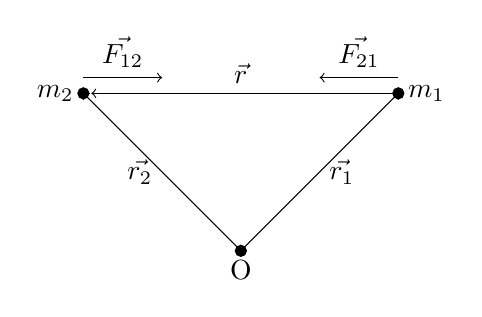
\begin{tikzpicture}

\draw[->] (0,0) -- (2,2);
\filldraw[black] (1,1) circle (0pt) node [anchor=west]{$\vec{r_1}$};

\draw[->] (0,0) -- (-2,2);
\filldraw[black] (-1,1) circle (0pt) node [anchor=east]{$\vec{r_2}$};

\filldraw[black] (2,2) circle (2pt) node [anchor=west]{$m_1$};
\filldraw[black] (-2,2) circle (2pt) node [anchor=east]{$m_2$};
\filldraw[black] (0,0) circle (2pt) node [anchor=north]{O};
\filldraw[->] (2,2) -- (-1.9,2);
\filldraw[black] (0,2) circle (0pt) node [anchor=south]{$\vec{r}$};

\draw[->] (2,2.2) -- (1,2.2);
\filldraw[black] (1.5,2.2) circle (0pt) node [anchor=south]{$\vec{F_{21}}$};

\draw[->] (-2,2.2) -- (-1,2.2);
\filldraw[black] (-1.5,2.2) circle (0pt) node [anchor=south]{$\vec{F_{12}}$};

\end{tikzpicture}
\caption[Two bodies interacting with some force]{Two bodies interacting with some force at some time}
\labfig{draw_1}
\end{marginfigure}


Using Newton 3rd Law we can explain the movement of this two objects by two equations:

\begin{equation}
    \label{newton_1}
    m_1 \frac{d^2\vec{r_1}}{dt^2} = f(r)\hat{r}
\end{equation}

\begin{equation}
    \label{newton_2}
    m_2 \frac{d^2\vec{r_2}}{dt^2} = - f(r)\hat{r}
\end{equation}

Let's add \ref{newton_1} and \ref{newton_2}, this is going to be useful later.

\begin{equation}
    \label{newton_1+2}
    m_1\frac{d^2\vec{r_1}}{dt^2} + m_2\frac{d^2\vec{r_2}}{dt^2} = 0
\end{equation}

We can not get anything from \ref{newton_1} and \ref{newton_2}, so we are going to transform this equations into something we can use to resolve them. First, we define the center of mass and their derivatives among time:

\begin{equation}
    \label{center_of_mass}
    \vec{r_{CM}}=\frac{m_1\vec{r_1} + m_2\vec{r_2}}{m_1 + m_2}
\end{equation}

\begin{equation}
    \label{velocity_center_of_mass}
    \vec{v_{CM}}=\frac{d}{dt}\vec{r_{CM}} = \frac{1}{m_1 + m_2}\left[m_1\frac{d\vec{r_1}}{dt} + m_2\frac{d\vec{r_2}}{dt}  \right]
\end{equation}

\begin{equation}
    \label{aceleration_center_of_mass}
    \vec{a_{CM}}=\frac{d}{dt}\vec{v_{CM}} = \frac{1}{m_1 + m_2}\left[m_1\frac{d^2\vec{r_1}}{dt^2} + m_2\frac{d^2\vec{r_2}}{dt^2}  \right]
\end{equation}

If we look at \ref{aceleration_center_of_mass} we can see something equal to the left term of \ref{newton_1+2} so we can say that the acceleration of the center of mass is zero, i.e. $\vec{a_{CM}} = 0$.

This mean that the center of mass moves with a constant velocity and we can define it's move as:

\begin{equation}
    \label{center_of_mass_2}
    \vec{r_{CM}}= R_{CM} + V_{CM} \cdot t
\end{equation}

Where $R_{CM}$ and $V_{CM}$ are constants defined by initial conditions. Knowing this we can make a change of the coordinates with the next assumption:

\begin{equation}
    \label{change_of_coordinates_1}
    \vec{r_{1}} = \vec{r_{1}'} + \vec{r_{CM}}
\end{equation}

\begin{equation}
    \label{change_of_coordinates_2}
    \vec{r_{2}} = \vec{r_{2}'} + \vec{r_{CM}}
\end{equation}

% Second Figure : Change of the coordinates

\begin{marginfigure}[-3cm]
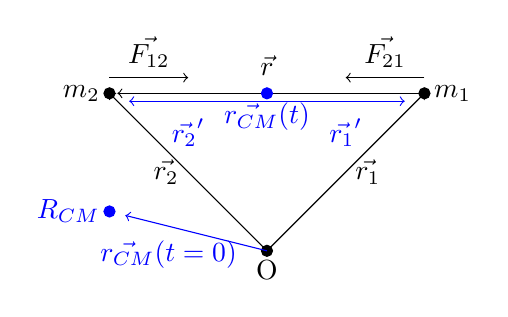
\begin{tikzpicture}

\draw[->] (0,0) -- (2,2);
\filldraw[black] (1,1) circle (0pt) node [anchor=west]{$\vec{r_1}$};

\draw[->] (0,0) -- (-2,2);
\filldraw[black] (-1,1) circle (0pt) node [anchor=east]{$\vec{r_2}$};

\filldraw[black] (2,2) circle (2pt) node [anchor=west]{$m_1$};
\filldraw[black] (-2,2) circle (2pt) node [anchor=east]{$m_2$};
\filldraw[black] (0,0) circle (2pt) node [anchor=north]{O};
\filldraw[->] (2,2) -- (-1.9,2);
\filldraw[black] (0,2.1) circle (0pt) node [anchor=south]{$\vec{r}$};

\draw[->] (2,2.2) -- (1,2.2);
\filldraw[black] (1.5,2.2) circle (0pt) node [anchor=south]{$\vec{F_{21}}$};

\draw[->] (-2,2.2) -- (-1,2.2);
\filldraw[black] (-1.5,2.2) circle (0pt) node [anchor=south]{$\vec{F_{12}}$};

% Change
\draw[->, blue] (0,0) -- (-1.8,0.45);
\filldraw[blue] (-2,0.5) circle (2pt) node [anchor=east]{${R_{CM}}$};
\filldraw[blue] (-1.25,0.25) circle (0pt) node [anchor=north]{${\vec{r_{CM}}(t = 0)}$};

\filldraw[blue] (0,2) circle (2pt) node [anchor=north]{${\vec{r_{CM}}(t)}$};

\draw[->, blue] (0,1.9) -- (1.75,1.9);
\filldraw[blue] (1,1.8) circle (0pt) node [anchor=north]{$\vec{r_1}'$};

\draw[->, blue] (0,1.9) -- (-1.75,1.9);
\filldraw[blue] (-1,1.8) circle (0pt) node [anchor=north]{$\vec{r_2}'$};

\end{tikzpicture}
\caption[Two-body problem with new coordinates]{Two-body problem with the new coordinates}
\labfig{draw_2}
\end{marginfigure}

Now let's calculate the new center of mass $\vec{r_{CM}'}$ using \ref{change_of_coordinates_1} and \ref{change_of_coordinates_2}

\begin{equation}
    \label{cm_prima}
    \begin{split}
    \vec{r_{CM}'} & = \frac{m_1\vec{r_1'}+ m_2\vec{r_2'}}{m_1+m_2} \\
                  & = \frac{1}{m_1 + m_2} \left[ m_1(\vec{r_1}-\vec{r_{CM}}) + m_2(\vec{r_2}-\vec{r_{CM}})\right] \\
                  & = \vec{r_{CM}} - \frac{1}{m_1+m_2}\left[\vec{r_{CM}}(m_1+ m_2)\right]\\
                  & = \vec{r_{CM}} - \vec{r_{CM}} = 0 \hspace{2mm} \sidenote[][2mm]{The professor demonstrate the same but with the expression for \vec{r_{CM}}, this is just another way I prefer.} 
    \end{split}              
\end{equation}

As it should be, our new center of mass is the origin for all time because our new referential system is moving with the center of mass. From this assumptions and using the definition of the new center of mass above we can get a new system of equations.

\begin{equation}
\label{sys_eq_1}
    \left\{
    \begin{array}{l}
        m_1\vec{r_1'} + m_2\vec{r_2'} = 0 \\
        \vec{r_1'} - \vec{r_2'} = \vec{r}
    \end{array}
    \right. =
    \left\{
    \begin{array}{l}
        \vec{r_1'} = \frac{m_2\vec{r}}{m_1+m_2} \\
        \vec{r_2'} = \frac{-m_1\vec{r}}{m_1+m_2}
    \end{array}
    \right.
\end{equation}

 We use what we obtain from \ref{sys_eq_1} in \ref{newton_1} and \ref{newton_2}. We can do this because the force does not change in this coordinates because only depend on r and this magnitude is still the same, i.e. $\vec{r}=\vec{r'}$.

\begin{equation}
\label{sys_eq_sol}
    m \frac{d^2\vec{r}}{dt^2} = f(r) \vec{r} 
\end{equation}

\marginnote[-2mm]{m is the reduce mass define as: \newline $ m = \frac{m_1 m_2}{m_1 + m_2}$}
\marginnote[1cm]{Normally we can use $m \approx m_2$ when $m_1 >> m_2$, some examples of this are Sun and Earth or proton and electron. With real values:\newline $m_{S-E} = \frac{m_S m_E}{m_S + m_E} \approx 5.96998 \cdot 10^{24}kg \aprox m_E$, where $m_S = 2 \cdot10^{30}kg, m_E = 5.97\cdot 10^{24}kg$}

We get the same equation from both equations.This expression will be useful to resolve the problem later. 

\section{The Angular Momentum}
\labsec{does}

We define the angular momentum as:

\begin{equation}
\label{ang_mom}
    \vec{L} = \vec{r} \times \vec{p} = m \vec{r} \times \frac{d\Vec{r}}{dt}
\end{equation}

We want to now how this quantity changes among time.

\begin{equation}
\label{ang_mom_dt}
    \frac{d\vec{L}}{dt} = m \frac{\vec{dr}}{dt} \times \frac{d\vec{r}}{dt} + m \vec{r} \times \frac{d^2\vec{r}}{dt^2} = 0 + \vec{r} \times f(r) \hat{r} = 0
\end{equation}

The law of the conservation of angular momentum says that the angular momentum of a system remains constant unless an external rotational force (torque) acts upon it.

As we just demonstrate the angular momentum vector is constant and we can redefine it as:

\begin{equation}
\label{ang_mom_2}
    \vec{L} = L \hat{z}
\end{equation}

The decision of L going through the $\hat{z}$ direction is going to be very resourceful.



\section{Cylindrical coordinates}
\labsec{does}

We need to choose a coordinate system. The problem become easy if we choose cylindrical coordinates.

\begin{equation}
\label{cylindrical}
\begin{split}
    &\vec{r} = \rho \hat{\rho} + z \hat{z} \\
    &\frac{d\vec{r}}{dt} = \frac{d\rho}{dt}\hat{\rho} + \rho \frac{d\phi}{dt}\hat{\phi}+\frac{dz}{dt}\hat{z} 
\end{split}
\end{equation}

\begin{marginfigure}[-2cm]
    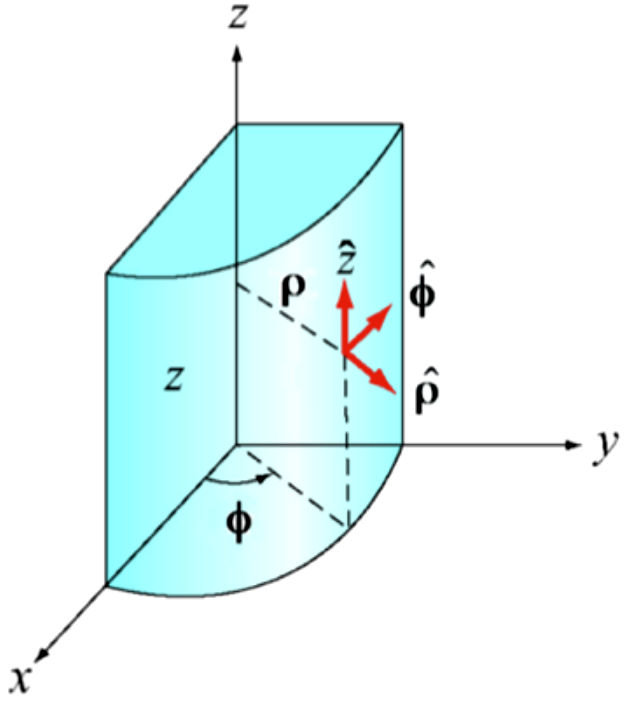
\includegraphics{cylindrical}
    \caption[Cylindrical coordinates]{Cylindrical coordinates.\\       \url{https://www.researchgate.net/publication/334148643/figure/fig1/AS:775915730649091@1562004134358/Diagram-of-a-standard-cylindrical-coordinate-system-with-radius-r-azimuth-ph-and-height.jpg}}
    \labfig{margincylind}
\end{marginfigure}

If we use \ref{cylindrical} in \ref{ang_mom_dt} we can look at $\Vec{L}$ components 

\begin{equation}
\label{cylindrical}
\begin{split}
    \vec{L} = & m (\rho \hat{\rho} + z \hat{z}) \times \left(\frac{d\rho}{dt}\hat{\rho} + \rho \frac{d\phi}{dt}\hat{\phi}+\frac{dz}{dt}\hat{z}\right) = \\
              & - m z \rho \frac{d\phi}{dt}\hat{\rho} + m\left(z\frac{d\rho}{dt}-\rho\frac{dz}{dt}\right)\hat{\phi}+ m \rho^2\frac{d\phi}{dt}\hat{z}
    \end{split}
\end{equation}

Using the definition in \ref{ang_mom_2} and our new equation we get 4 different equations if we compare the angular momentum in each direction.

\begin{equation}
    \label{sys_ang_mom}
    \begin{split}
    &1. \hspace{30} L \neq 0 \\
    &2. \hspace{30}m z \rho \frac{d\phi}{dt} = 0 \\
    &3. \hspace{30}m \left( z \frac{d\rho}{dt} - \rho \frac{dz}{dt} \right) = 0 \\
    &4. \hspace{30}m \rho^2\frac{d\phi}{dt} = L
    \end{split}
\end{equation}

This gives you a lot of information:

\begin{itemize}
    \item $m \neq 0$
    \item $\rho \neq 0$
    \item $\frac{d\phi}{dt} \neq 0$
    \item $z = 0$
    \item $\frac{d\phi}{dt} = \frac{L}{m\rho^2}$
    
\end{itemize}

This equations not only give us a fixed value of z it also give us that in the system we choose the value for z is 0 for all time. We also can get a relation between the derivative of $\phi$ and $\rho$ we are going to use this later to resolve the problem. 

If z=0 we can redefine $\vec{r}$ from \ref{cylindrical}.

\begin{equation}
    \label{from_r_to_rho}
    \begin{split}
        &\vec{r} = \vec{\rho} = \rho\hat{\rho} \\
        &\frac{d^2\vec{\rho}}{dt^2} = \left[ \frac{d^2\rho}{dt^2} -\rho\left(\frac{d\phi}{dt}\right)^2 \right]\hat{\rho} + \left[2\frac{d\rho}{dt}\frac{d\phi}{dt} +\rho\frac{d^2\phi}{dt^2} \right]\hat{\phi}
    \end{split}
\end{equation}

We loose the therm that goes in the $\hat{\phi}$ direction because is zero. We can see this in two different ways:

\begin{itemize}
    \item Now our force $F = f(r)\hat{r} = f(\rho)\hat{\rho}$ because \ref{from_r_to_rho} so the second derivative of $\Vec{\rho}$ only can have a component in the $\hat{\rho}$ direction.
    \item If we calculate what we have in the $\hat{\phi}$ component using some notions in derivatives and \ref{sys_ang_mom} we would get 0  \sidenote[][2cm]{$2\frac{d\rho}{dt}\frac{d\phi}{dt} +\rho\frac{d^2\phi}{dt^2} = \frac{d}{dt}\left(\rho^2\frac{d\phi}{dt}\right)= \frac{d}{dt}\left(\frac{L}{m}\right) = 0$, because both L and m are constants.}
\end{itemize}



If we return to \ref{sys_eq_sol} with everything we learnt we can get something very interesting, an scalar equation.

\begin{equation}
    \label{scalar_eq}
    m\left[ \frac{d^2\rho}{dt^2}-\rho\left(\frac{d\phi}{dt}\right)^2 \right] = f(\rho)
\end{equation}

We get a scalar equation with two variables $\rho$ and $\phi$, but we can use \ref{sys_ang_mom} as before and reduce everything to an one variable scalar equation.

\begin{equation}
    \label{solution_1}
    m\left[ \frac{d^2\rho}{dt^2}-\rho\frac{L^2}{m^2\rho^4}\right] = f(\rho) = -\frac{d\nu(\rho)}{d\rho}
\end{equation}

We can put everything in one side of the equation and multiply both sides by a factor $\frac{d\rho}{dt}$

\begin{equation} \label{solution_2}
    \begin{split}
    & m \frac{d^2\rho}{dt^2} \frac{d\rho}{dt} - \frac{d}{dt} \left( \frac{L^2}{m\rho^3} \right) + \frac{d}{dt} \frac{d\nu(\rho)}{d\rho} = 0 \\
    & \frac{d}{dt} \left(\frac{1}{2}m\left(\frac{d\rho}{dt}\right)^2+\frac{L^2}{2m\rho^2}+ \nu(\rho) \right) = 0
    \end{split}
\end{equation}

We know that this magnitude inside the brackets is constant during the time, this magnitude is the total energy (E) but we can divide this energy in three:

\begin{description}
    \item [Linear Kinetic Energy] $K = \frac{1}{2}m(\frac{d\rho}{dt})^2$
    \item [Angular Kinetic Energy] $K_{\alpha} = \frac{L^2}{2m\rho^2}$
    \item [Potential Energy] $\nu(\rho) = \frac{-k}{r}$   \sidenote[][2mm]{This is what we usually use as potential energy because it appears in nature. Ex: Newton Gravity Law and Coulomb Law}
\end{description}
     
\section{Potential wells}
\labsec{does}

We are going to study the angular kinetic energy and the potential energy (both are functions of $\rho$), we call the addition of these two energies \textbf{Effective potential}

\begin{marginfigure}
    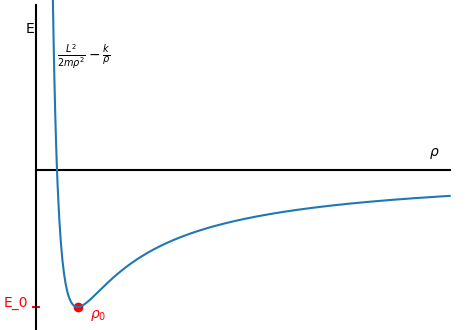
\includegraphics{images/General_Potential_Well.png}
    \caption[Effective Potential]{Effective Potential}
    \labfig{marginfigeff}
\end{marginfigure}

In \reffig{marginfigeff} we can see many things:

\begin{itemize}
    \item The function have a minimum that is the lowest possible total energy because the linear kinetic energy is always greater or equal to 0, i. e. $K\geq0$. This energy represents a circular motion.
    
    \item If we have a higher energy but still negative, the movement is an elliptical motion with two values that are the nearest and the furthest point in the ellipse.
    
    \item If the motion is higher than 0 the motion is not more a close orbit and then the motion is an hyperbola.
    
    \item If the total energy is 0, the motion is in the limit between a close and an open orbit and the movement is a parable.
\end{itemize}

In the next section we are going to give real values to this magnitudes.

\section{Physical Examples}
\labsec{does}

\textbf{1. Earth-Sun problem:} If we take the Earth and the Sun as our two bodies we need to know some values. We already know the reduce mass from the previous section. The k value of the potential energy is $ k = GM_Sm_E$, we know this value from Newton´s Gravitational Law.

\begin{itemize}
    \item $m_E = 2 \cdot 10{30} kg$
    \item $M_S = 5.97\cdot 10^{24} kg$
    \item $G = 6.67 \cdot 10^{11} Nm^2/kg^2$
\end{itemize}

The total energy of the system is:

\begin{equation}
\label{energy_E-S}
    E = \frac{1}{2}m\left(\frac{d\rho}{dt}\right)^2+\frac{L^2}{2m\rho^2}+ \frac{ - G M_S m_E}{\rho} 
\end{equation}

We can see in \reffig{marginfig_ES} that if we represent $U = K_{\alpha}+\nu(\rho)$ against $\rho$ we get a similar function to the one in \reffig{marginfigeff}, but we can see in the axis that we have large energies and distances. That is reasonable if we think that we are working with massive objects as planets.

\begin{marginfigure}
    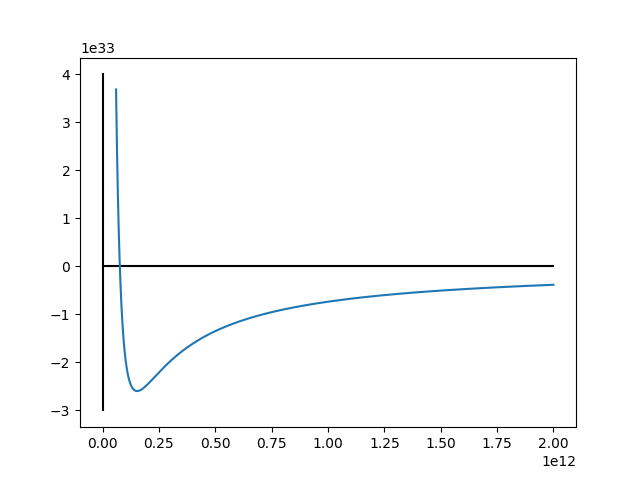
\includegraphics{images/E-S_Potential_Well.png}
    \caption[Effective Potential for Earth-Sun]{Effective Potential for Earth-Sun}
    \labfig{marginfig_ES}
\end{marginfigure}

We can calculated now the minimum energy the Earth-Sun system can have in which, the Earth would orbit by a circular motion. 

To calculate this energy we need to calculate first the value of $\rho$ for this minimum energy ($\rho_{min}$). This value can be found by matching the first derivative of the function U($\rho$) to 0

\begin{equation}
    \label{Der_Ueff}
    \begin{split}
    &\frac{dU}{d\rho} = \frac{d}{d\rho}\left[ \frac{L^2}{2m\rho^2}+ \frac{ - G M_S m_E}{\rho}\right]=\\
    &\frac{-L^2}{m\rho^3}+\frac{G M_S m_E}{\rho^2}
    \end{split}
\end{equation}

If we match \ref{Der_Ueff} to 0 and solve for $\rho$ we get $\rho_{min}$

\begin{equation}
    \label{rho_min_ES}
    \begin{split}
    &\frac{-L^2}{m\rho^3}+\frac{G M_S m_E}{\rho^2} = 0\\
    &\frac{G M_S m_{E}^2\rho - L^2}{m_E\rho^3} = 0\\
    &\rho_{min} = \frac{L^2}{G M_S m_{E}^2}
    \end{split}
\end{equation}

If we use \ref{rho_min_ES} in \ref{energy_E-S} knowing that our minimum energy implies K = 0, we get the minimum energy possible.

\begin{equation}
    \label{energy_min_ES}
    E = -\frac{1}{2}\frac{G^2M_{S}^2m_{E}^3}{L^2} = -\frac{1}{2}\frac{G M_S m_{E}}{\rho_{min}}=\frac{1}{2}\nu(\rho_{min})
\end{equation}

If we look into the equation \ref{energy_min_ES} we can demonstrate that the minimum energy is a half of the potential energy. 

\textbf{2. Electron-Proton problem:} If we take a proton and an electron we can do the same as before knowing their masses. The problem is very similar, just with different conditions. The reduce mass is going to be the mass of the electron because it is much less than the mass of the proton.

\begin{itemize}
    \item $m_e = 9.11 \cdot 10{-31} kg$
    \item $m_p = 1.67\cdot 10^{-27} kg$
    \item $G = 6.67 \cdot 10^{11} kg$
\end{itemize}

The total energy of the system is:

\begin{equation}
\label{energy_E-P_mass}
    E = \frac{1}{2}m\left(\frac{d\rho}{dt}\right)^2+\frac{L^2}{2m\rho^2}+ \frac{ - G M_p m_e}{\rho} 
\end{equation}

\begin{marginfigure}
    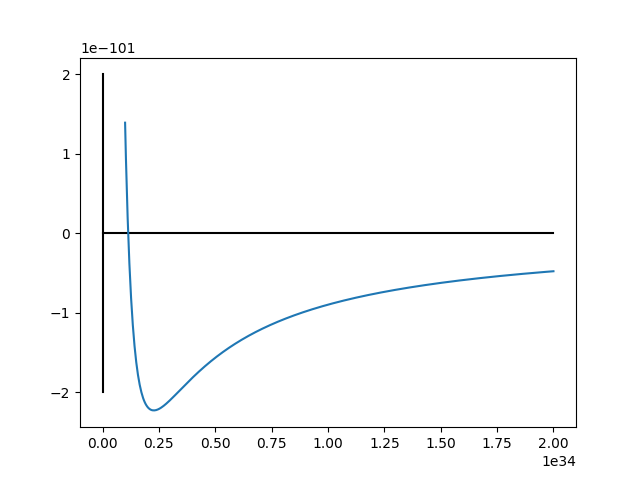
\includegraphics{images/E-P_Potential_Well.png}
    \caption[Effective Potential for Electron-Proton]{Effective Potential for Electron-Proton}
    \labfig{marginfig_EP}
\end{marginfigure}

We can see in \reffig{marginfig_EP} that if we represent $U = K_{\alpha}+\nu(\rho)$ against $\rho$ we get a similar function to \reffig{marginfigeff}, but if we focus in the axis we can see that we have very low energies. That is reasonable if we think that we are working with particles that have very little mass.

I'm not going to do all we did before. In this case, because the energy is so low, is not interesting to study it. But there is another potential that affects electron and proton, the electric potential.

\textbf{3. Electron-Proton problem with Electric Potential:} In this case we need to define the charges of the proton and the electron. Also we need to define a new potential, where $ k = \frac{Ze^2}{4\pi\epsilon_0} $ where Z is the atomic number, e is the charge of the electron  \sidenote[][1mm]{This value was discovered by the Nobel Price Robert Andrews Millikan by his experiment called: Millikan oil drop experiment} and $\epsilon_0$ is the permittivity of free space.

\begin{itemize}
    \item $e = 1.6 \cdot 10^{-19} \cdot 10{30} kg$
    \item $\epsilon_0 = 8.85 \cdot 10^{-12} kg$
\end{itemize}

The total energy of the system is:

\begin{equation}
\label{energy_E-P_elec}
    E = \frac{1}{2}m\left(\frac{d\rho}{dt}\right)^2+\frac{L^2}{2m\rho^2}+ \frac{-Ze^2}{4\pi\epsilon_0\rho} 
\end{equation}

If we look at \reffig{marginfig_EP_elec} and compare it with \reffig{marginfig_EP} we can see a high difference in the Energy scale. This means that the electrical force is much stronger than the gravitational force.

\begin{marginfigure}
    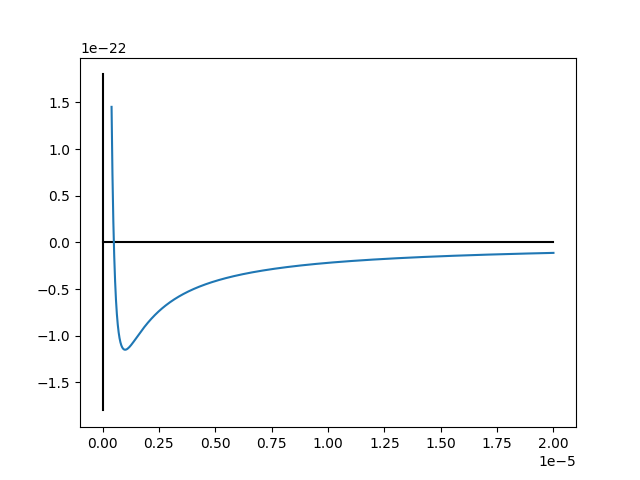
\includegraphics{images/E-P_elec_Potential_Well.png}
    \caption[Effective Potential for Electron-Proton (Electric Potential)]{Effective Potential for Electron-Proton (Electric Potential)}
    \labfig{marginfig_EP_elec}
\end{marginfigure}

We can calculated now the minimum energy the Electron-Proton system can have in which, the electron would orbit by a circular motion around the proton. 

To calculate this energy we need to calculate first the value of $\rho$ for this minimum energy ($\rho_{min}$). This value can be found by matching the first derivative of the function in \reffig{marginfig_ES} to 0

\begin{equation}
    \label{Der_Ueff}
    \begin{split}
    &\frac{dU}{d\rho} =\frac{d}{d\rho}\left[ \frac{L^2}{2m\rho^2}+ \frac{ -Ze^2}{\rho}\right]=\\
    &\frac{-L^2}{m\rho^3}+\frac{-Ze^2}{4\pi\epsilon_0\rho^2}
    \end{split}
\end{equation}

If we match \ref{Der_Ueff} to 0 and solve for $\rho$ we get $\rho_{min}$.

\begin{equation}
    \label{rho_min}
    \begin{split}
    &\frac{-L^2}{m\rho^3}+\frac{Ze^2}{4\pi\epsilon_0\rho^2} = 0\\
    &Ze^2m\rho - 4 L^2\pi\epsilon_0 = 0\\
    &\rho_{min} = \frac{4L^2\pi\epsilon_0}{Ze^2m}
    \end{split}
\end{equation}

We can also get the square of the angular momentum as a function of $\rho$.

\begin{equation}
    \label{L_min}
    L^2 = \frac{m\rho_{min}Ze^2}{4\pi\epsilon_0}
\end{equation}

Now, we have two different expressions for the minimum energy.

\begin{equation}
    \label{E_min_EP}
    \begin{split}
    &1) E_{min} = -\frac{Ze^2}{8\pi\epsilon_0\rho^2}\\
    &2) E_{min} = -\frac{Z^2e^4m}{2(4\pi\epsilon_0)^2}\frac{1}{L^2}     
    \end{split}
\end{equation}

Looking at the first expression we have the same as the Earth-Proton problem, we get that the minimum energy is half of the potential energy. 

The second expression is even more interesting because after measure the length wave of light from an hydrogen atom, Bohr discovered that L was proportional to the energy level of the atom (n). Later they found that the relation is:

\begin{equation}
    \label{L_min}
    L = hn  
\end{equation}
\marginnote{h is known as the Plank constant. \\
$h\approx 6.63\cdot10^{-34}$}

\section{Rotation and angular momentum}
\labsec{does}

To finished this chapter we are going to talk about something that is very interesting and purely mathematical. 

We know that the rotation in 3D is not commutative and we also know that the definition of the module of $\vec{L}$ is

\begin{equation}
    \label{module_L}
    L^2=|\Vec{L}|^2=L_{x}^2+L_{y}^2+L_{z}^2
\end{equation}

This means that we can have multiple solutions for L using rotations.

We define a vector |j,m > where j is the representation and m is the bases vector of the representation. Then we get this relations:

\begin{equation}
\label{jm_vec}
    \begin{split}
        &1) L^2| j,m > = j(j+1)| j,m >\\
        &2) L_z| j,m > = m | j,m >
    \end{split}
\end{equation}

I'm not proving anything, we will talk about this later.

% The \Class{kaobook} class focuses more about the document structure than 
% about the style. Indeed, it is a well-known \LaTeX\xspace principle that 
% structure and style should be separated as much as possible (see also 
% \vrefsec{doesnot}). This means that this class will only provide 
% commands, environments and in general, the opportunity to do things, 
% which the user may or may not use. Actually, some stylistic matters are 
% embedded in the class, but the user is able to customise them with ease.

% The main features are the following:

% \begin{description}
% 	\item[Page Layout] The text width is reduced to improve readability 
% 	and make space for the margins, where any sort of elements can be 
% 	displayed.
% 	\item[Chapter Headings] As opposed to Tufte-Latex, we provide a 
% 	variety of chapter headings among which to choose; examples will be 
% 	seen in later chapters.
% 	\item[Page Headers] They span the whole page, margins included, and, 
% 	in twoside mode, display alternatively the chapter and the section 
% 	name.\sidenote[][-2mm]{This is another departure from Tufte's 
% 	design.}
% 	\item[Matters] The commands \Command{frontmatter}, 
% 	\Command{mainmatter} and \Command{backmatter} have been redefined in 
% 	order to have automatically wide margins in the main matter, and 
% 	narrow margins in the front and back matters. However, the page 
% 	style can be changed at any moment, even in the middle of the 
% 	document.
% 	\item[Margin text] We provide commands \Command{sidenote} and 
% 	\Command{marginnote} to put text in the 
% 	margins.\sidenote[][-2mm]{Sidenotes (like this!) are numbered while 
% 	marginnotes are not}
% 	\item[Margin figs/tabs] A couple of useful environments is 
% 	\Environment{marginfigure} and \Environment{margintable}, which, not 
% 	surprisingly, allow you to put figures and tables in the margins 
% 	(\cfr \reffig{marginmonalisa}).
% 	\item[Margin toc] Finally, since we have wide margins, why don't add 
% 	a little table of contents in them? See \Command{margintoc} for 
% 	that.
% 	\item[Hyperref] \Package{hyperref} is loaded and by default we try 
% 	to add bookmarks in a sensible way; in particular, the bookmarks 
% 	levels are automatically reset at \Command{appendix} and 
% 	\Command{backmatter}. Moreover, we also provide a small package to 
% 	ease the hyperreferencing of other parts of the text.
% 	\item[Bibliography] We want the reader to be able to know what has 
% 	been cited without having to go to the end of the document every 
% 	time, so citations go in the margins as well as at the end, as in 
% 	Tufte-Latex. Unlike that class, however, you are free to customise 
% 	the citations as you wish.
% \end{description}

% \begin{marginfigure}[-5.5cm]
% 	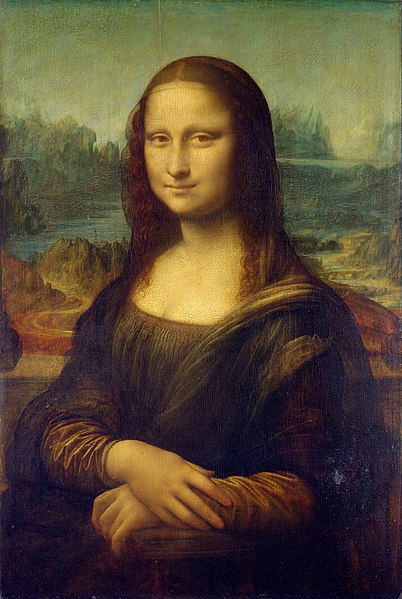
\includegraphics{monalisa}
% 	\caption[The Mona Lisa]{The Mona Lisa.\\ 
% 	\url{https://commons.wikimedia.org/wiki/File:Mona_Lisa,_by_Leonardo_da_Vinci,_from_C2RMF_retouched.jpg}}
% 	\labfig{marginmonalisa}
% \end{marginfigure}

% The order of the title pages, table of contents and preface can be 
% easily changed, as in any \LaTeX\ document. In addition, the class is 
% based on \KOMAScript's \Class{scrbook}, therefore it inherits all the 
% goodies of that.

% \section{What This Class Does Not Do}
% \labsec{doesnot}

% As anticipated, further customisation of the book is left to the user. 
% Indeed, every book may have sidenotes, margin figures and so on, but 
% each book will have its own fonts, toc style, special environments and 
% so on. For this reason, in addition to the class, we provide only 
% sensible defaults, but if these features are not needed, they can be 
% left out. These special packages are located in the \Path{style} 
% directory, which is organised as follows:

% \begin{description}
% 	\item[kao.sty] This package contains the most important definitions 
% 	of macros and specifications of page layout. It is the heart of the 
% 	\Class{kaobook}.
% 	\item[kaobiblio.sty] Contains commands to add citations and 
% 	customise the bibliography.
% 	\item[packages.sty] Loads additional packages to decorate the 
% 	writing with special contents (for instance, the \Package{listing} 
% 	package is loaded here as it is not required in every book). There 
% 	are also defined some useful commands to print the same words always 
% 	in the same way, \eg latin words in italics or \Package{packages} in 
% 	verbatim.
% 	\item[kaorefs.sty] Some useful commands to manage labeling and 
% 	referencing, again to ensure that the same elements are referenced 
% 	always in a consistent way.
% 	\item[environments.sty] Provides special environments, like boxes. 
% 	Both simple and complex environments are available; by complex we 
% 	mean that they are endowed with a counter, floating and can be put 
% 	in a special table of contents.\sidenote[][-2mm]{See 
% 	\vrefch{mathematics} for some examples.}
% 	\item[theorems.sty] The style of mathematical environments. 
% 	Actually, there are two such packages: one is for plain theorems,
% 	\ie the theorems are printed in plain text; the other uses 
% 	\Package{mdframed} to draw a box around theorems. You can plug the 
% 	most appropriate style into its document.
% \end{description}

% \marginnote[2mm]{The audacious users might feel tempted to edit some of 
% these packages. I'd be immensely happy if they sent me examples of what 
% they have been able to do!}

% In the rest of the book, I shall assume that the reader is not a novice 
% in the use of \LaTeX, and refer to the documentation of the packages 
% used in this class for things that are already explained there. 
% Moreover, I assume that the reader is willing to make minor edits to the 
% provided packages for styles, environments and commands, if he or she 
% does not like the default settings.

% \section{How to Use This Class}

% Either if you are using the template from 
% \href{http://latextemplates.org/template/kaobook}{latextemplates}, or if 
% you cloned the GitHub 
% \href{https://www.github.com/fmarotta/kaobook}{repository}, there are 
% infinite ways to use the \Class{kaobook} class in practice, but we will 
% discuss only two of them. The first is to find the \Path{main.tex} file 
% which I used to write this book, and edit it; this will probably involve 
% a lot of text-deleting, copying-and-pasting, and rewriting. The second 
% way is to start almost from scratch and use the \Path{skeleton.tex} 
% file, which is a cleaned-up version of the \Path{main.tex}; even if you 
% choose the second way, you may find it useful to draw inspiration from 
% the \Path{main.tex} file.

% To compile the document, assuming that its name is \Path{main.tex}, you 
% will have to run the following sequence of commands:

% \begin{lstlisting}[style=kaolstplain,linewidth=1.5\textwidth]
% pdflatex main # Compile template
% makeindex main.nlo -s nomencl.ist -o main.nls # Compile nomenclature
% makeindex main # Compile index
% biber main # Compile bibliography
% makeglossaries main # Compile glossary
% pdflatex main # Compile template again
% pdflatex main # Compile template again
% \end{lstlisting}

% You may need to compile the template some more times in order for some 
% errors to disappear. For any support requests, please ask a question on 
% \url{tex.stackexchange.org} with the tag \enquote{kaobook}, open an 
% issue on GitHub, or contact the author via e-mail.
